
\documentclass[12pt,a4paper]{report}%especifica o tipo de documento que tenciona escrever: carta, artigo, relatório... neste caso é um relatório
% [11pt,a4paper] Define o tamanho principal das letras do documento. caso não especifique uma delas, é assumido 10pt
% a4paper -- Define o tamanho do papel.

\usepackage[portuges]{babel}%Babel -- irá activar automaticamente as regras apropriadas de hifenização para a língua todo o
                                   %-- o texto gerado é automaticamente traduzido para Português.
                                   %  Por exemplo, “chapter” irá passar a “capítulo”, “table of contents” a “conteúdo”.
                                   % portuges -- específica para o Português.
\usepackage[utf8]{inputenc} % define o encoding usado texto fonte (input)--usual "utf8" ou "latin1

\usepackage{graphicx} %permite incluir graficos, tabelas, figuras
\usepackage{url} % para utilizar o comando \url{}
\usepackage[pdftex]{hyperref} % transformar as referências internas do seu documento em hiper-ligações.
\usepackage{enumerate} %permite escolher, nas listas enumeradas, se os iems sao marcados com letras ou numeros-romanos em vez de numeracao normal

%\usepackage{apalike} % gerar biliografia no estilo 'named' (apalike)

\usepackage{xcolor} % Para escrever em cores
\usepackage{soul} % Para sombrear um texto (highlighter)
\sethlcolor{pink}

\usepackage{multirow} %tabelas com multilinhas
\usepackage{array} %formatação especial de tabelas em array
\usepackage{float}
\usepackage[pdftex]{hyperref} % transformar as referências internas do seu documento em hiper-ligações.

%Exemplos de fontes -- nao e vulgar mudar o tipo de fonte
%\usepackage{tgbonum} % Fonte de letra: TEX Gyre Bonum
%\usepackage{lmodern} % Fonte de letra: Latin Modern Sans Serif
%\usepackage{helvet}  % Fonte de letra: Helvetica
%\usepackage{charter} % Fonte de letra:Charter

\definecolor{saddlebrown}{rgb}{0.55, 0.27, 0.07} % para definir uma nova cor, neste caso 'saddlebrown'

\usepackage{listings}  % para utilizar blocos de texto verbatim no estilo 'listings'
%paramerização mais vulgar dos blocos LISTING - GENERAL
\lstset{
	basicstyle=\small, %o tamanho das fontes que são usadas para o código
	numbers=left, % onde colocar a numeração da linha
	numberstyle=\tiny, %o tamanho das fontes que são usadas para a numeração da linha
	numbersep=5pt, %distancia entre a numeração da linha e o codigo
	breaklines=true, %define quebra automática de linha
    frame=tB,  % caixa a volta do codigo
	mathescape=true, %habilita o modo matemático
	escapeinside={(*@}{@*)} % o que escrever dentro destas marcas é aceite e processado como LaTeX
}
%
\lstset{ 
	language=Python,% choose the language of the code
        basicstyle=\ttfamily\footnotesize,		% the size of the fonts that are used for the code
	keywordstyle=\bfseries,					% set the keyword style
	%numbers=left,							% where to put the line-numbers
	numberstyle=\scriptsize,				% the size of the fonts that are used for the line-numbers
	stepnumber=1,% the step between two line-numbers. If it's 1 each line
	numbers=none,
        frame=lines,
        resetmargins=true,										% will be numbered
	numbersep=5pt,							% how far the line-numbers are from the code
	backgroundcolor=\color{white},			% choose the background color. You must add \usepackage{color}
	showspaces=false,						% show spaces adding particular underscores
	showstringspaces=false,					% underline spaces within strings
	showtabs=false,							% show tabs within strings adding particular underscores
	frame=none,								% adds a frame around the code
	%abovecaptionskip=-.8em,
	%belowcaptionskip=.7em,
	tabsize=1,								% sets default tabsize to 2 spaces
	captionpos=b,							% sets the caption-position to bottom
	breaklines=true,						% sets automatic line breaking
	breakatwhitespace=false,				% sets if automatic breaks should only happen at whitespace
	title=\lstname,							% show the filename of files included with \lstinputlisting;
											% also try caption instead of title
	escapeinside={\%*}{*)},					% if you want to add a comment within your code
	morekeywords={*,...}					% if you want to add more keywords to the set
}

\lstdefinestyle{withlines}{
    language=Python,
    frame=lines, % Linhas no topo e na base
    rulecolor=\color{gray}, % Linha cinza
    framexleftmargin=5pt,
    framexrightmargin=5pt
}

\usepackage{xspace} % deteta se a seguir a palavra tem uma palavra ou um sinal de pontuaçao se tiver uma palavra da espaço, se for um sinal de pontuaçao nao da espaço

\parindent=0pt %espaço a deixar para fazer a  indentação da primeira linha após um parágrafo
\parskip=2pt % espaço entre o parágrafo e o texto anterior

\setlength{\oddsidemargin}{-1cm} %espaço entre o texto e a margem
\setlength{\textwidth}{18cm} %Comprimento do texto na pagina
\setlength{\headsep}{-1cm} %espaço entre o texto e o cabeçalho
\setlength{\textheight}{23cm} %altura do texto na pagina

% comando '\def' usado para definir abreviatura (macros)
% o primeiro argumento é o nome do novo comando e o segundo entre chavetas é o texto original, ou sequência de controle, para que expande
\def\darius{\textsf{Darius}\xspace}
\def\antlr{\texttt{AnTLR}\xspace}
\def\pe{\emph{Publicação Eletrónica}\xspace}
\def\titulo#1{\section{#1}}    %no corpo do documento usa-se na forma '\titulo{MEU TITULO}'
\def\super#1{{\em Supervisor: #1}\\ }
\def\area#1{{\em \'{A}rea: #1}\\[0.2cm]}
\def\resumo{\underline{Resumo}:\\ }

%\input{LPgeneralDefintions} %permite ler de um ficheiro de texto externo mais definições

\title{Computação Gráfica (3º ano de LCC)\\
       \textbf{2ª Fase} \\ Relatório de Desenvolvimento\\
       \textbf{ Grupo 18 }
       } %Titulo do documento
       
%\title{Um Exemplo de Artigo em \LaTeX}
\author{Eduardo Pereira\\ (A70619) \and Diogo Coelho \\ (A100092)
         \and Pedro Oliveira\\ (A97686) \and João Barbosa\\ (A100054)
       } %autores do documento
\date{\today} %data

\begin{document} % corpo do documento
\maketitle % apresentar titulo, autor e data

\begin{abstract}  % resumo do documento

Este relatório descreve o desenvolvimento da primeira fase de um projeto, desenvolvido no âmbito da Unidade Curricular de Computação Gráfica, do 3º ano da Licenciatura em Ciências da Computação, na Universidade do Minho.\newline 
\\ Este projeto consiste na implementação de duas grandes componentes: um \textbf{generator} e um \textbf{engine}, que em conjunto produzem figuras geométricas visíveis num espaço 3D.\\ \newline
O \textbf{generator} é responsável pela geração dos vértices relativos a cada figura, enquanto que o \textbf{engine} trata da renderização dos objetos no espaço. \\
\end{abstract}

\tableofcontents % Insere a tabela de indice
\listoffigures % Insere a tabela de indice figuras
%\listoftables % Insere a tabela de indice tabelas

\chapter{Introdução} \label{chap:intro} %referência cruzada

No âmbito da Unidade Curricular de Computação Gráfica, foi-nos proposto, pelo docente, a implementação de um sistema capaz de desenhar figuras num espaço 3D. \newline
\\ O objetivo desta primeira fase é desenvolver um sistema para gerar figuras geométricas de forma que estes objetos sejam desenhados com base nas configurações de uma câmara definidas num ficheiro  \textbf{\texttt{XML}}.\\
Este projeto é desenvolvido utilizando a linguagem \textbf{\texttt{C++}} e recorrendo à ferramenta \textbf{\texttt{OpenGL}} para o desenho das várias figuras geométricas. \\
\\ Neste relatório será apresentada a nossa interpretação do problema, assim como as abordagens adotadas ao longo da implementação deste projeto.
\\ 

\newpage
\titulo{Estrutura do Relatório}
De forma a facilitar a leitura e compreensão deste documento, nesta secção será explicada a sua estrutura e o conteúdo de cada um dos capítulos resumido e explicado.

\begin{itemize}
    \item \textbf{Capítulo ~\ref{chap:intro}} - Definição do Sistema, que consiste em: Introduzir e descrever a contextualização do projeto desenvolvido, assim como os objetivos a atingir com o mesmo.
    \item \textbf{Capítulo ~\ref{chap:analiseEspecificacao}} - Análise e Especificação: Descrever informalmente o problema, indicando o que se espera ser possível fazer.
    \item \textbf{Capítulo ~\ref{chap:instructions}} - Instruções de Utilização: Instruções para compilar e executar os programas do projeto
    \item \textbf{Capítulo ~\ref{chap:testes}} - Testes: Neste capítulo são apresentados diversos testes realizados sobre o nosso programa
    \item \textbf{Capítulo ~\ref{chap:conclusao}} - Conclusão: Contém as últimas impressões acerca do projeto desenvolvido e oportunidades de trabalho futuro.
\end{itemize}

\chapter{Análise e Especificação} \label{chap:analiseEspecificacao} %capitulo e referencia cruzada
\section{Descrição informal do problema} \label{sec:descricaoProblema} 
%seccao e referencia cruzada
Esta fase do trabalho requer a criação de dois programas para a renderização de modelos geométricos. \par
O primeiro programa, \textbf{Generator}, tem como função gerar ficheiros que contêm os vértices das primitivas gráficas que vão ser utilizadas pelo outro programa \textbf{Engine}. Recebe como parâmetros os valores necessários para a criação dos modelos geométricos e armazena num ficheiro os vértices dos triângulos que definem as figuras. Com o gerador é possível obter os vértices dos triângulos para gerar as seguintes figuras: 
\begin{itemize}
  \item \textbf{Plano:} Um quadrado no eixo XZ, centrado na origem, subdividido nas direções X e Z.
  \item \textbf{Caixa:} Requer dimensão e o número de divisões por aresta, e está centrada na origem
  \item \textbf{Esfera:} Requer um raio, \textbf{slices} e \textbf{stacks}, e está centrada na origem
  \item \textbf{Cone:} Requer um raio para a base, altura, \textbf{slices} e \textbf{stacks}, e a base do cone está no eixo XZ.
\end{itemize}

O segundo programa, \textbf{Engine}, interpreta um ficheiro \textbf{\texttt{XML}} que contém os parâmetros para a composição da cena a renderizar, incluindo também a indicação dos modelos a desenhar. Deve ser utilizada a biblioteca \textbf{\texttt{tinyXML2}} para facilitar a leitura do ficheiro \textbf{\texttt{XML}}. 

Ambos os programas devem ser feitos em \textbf{\texttt{C++}}. 

\section{Proposta de resolução} \label{sec:descricaoProblema} 
%seccao e referencia cruzada

\subsection{Generator}
Este programa é responsável pela criação de representações tridimensionais de primitivas geométricas e guardá-las num ficheiro \textbf{.3d}. O gerador recebe como entrada um conjunto de parâmetros que especificam o tipo de figura geométrica a ser gerada, as suas dimensões e o nível de subdivisão da malha. Atualmente, são suportadas quatro figuras primitivas: plano, caixa, cone e esfera. O gerador valida os parâmetros fornecidos, garantindo que são numéricos e semanticamente corretos.

A geração de figuras baseia-se na decomposição das superfícies em triângulos, utilizando um sistema de coordenadas cartesianas tridimensionais. Cada figura é descrita num conjunto de triângulos definidos por três vértices, guardados num ficheiro \textbf{.3d}. Este ficheiro contém as coordenadas dos vértices gerados, para, à posteriori, serem interpretados pelo motor gráfico.

\begin{figure}[H]
    \centering
    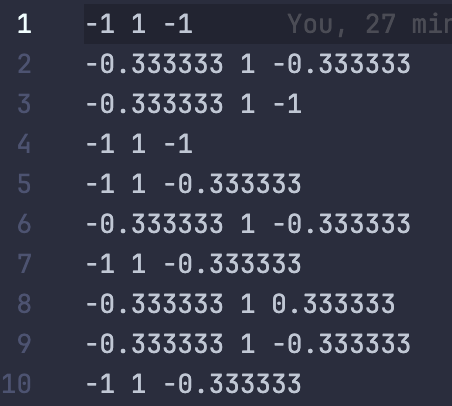
\includegraphics[width=0.5\linewidth]{images/PontosGerados.png}
    \caption{Excerto de um ficheiro \textbf{.3d} gerado}
    \label{fig:pontos-gerados}
\end{figure}

Cada primitiva geométrica segue um algoritmo específico para a sua criação:

\begin{itemize}
  \item \textbf{Plano}: é subdividido em quadrados com base no número de divisões especificado (\textbf{slices}). Cada quadrado é representada por dois triângulos. 
  \item \textbf{Caixa}: composta por seis faces, cada uma subdividida de forma semelhante ao plano.
  \item \textbf{Cone}: gerado a partir de um círculo base e de um vértice superior, subdividido em fatias (\textbf{slices}) ao longo da circunferência e em camadas (\textbf{stacks}) ao longo da altura.
  \item \textbf{Esfera}: construída utilizando coordenadas esféricas, onde os meridianos (\textbf{slices}) e paralelos (\textbf{stacks}) são utilizados para definir os vértices e os triângulos que compõem a superfície esférica.
\end{itemize}



A implementação do gerador está dividida em dois ficheiros principais:
\begin{itemize}
    \item \textbf{generator.cpp}: Responsável pelo \textbf{parsing} dos argumentos, seleção da figura a gerar e invocação das funções adequadas para cada tipo de primitiva.
    \item \textbf{generatorAux.cpp}: Contém as funções específicas para a geração das diferentes figuras geométricas. Cada função calcula os vértices e escreve os resultados num ficheiro.
\end{itemize}

\subsection{Exemplos Figuras Geradas}

\textbf{Plane} \\

O plano é gerado no eixo XZ, i.e, Y=0. É dividido numa matriz de quadrados com base no número de divisões, i.e , o número de \textbf{slices}. Vamos supor que o número de \textbf{slices} é \(i\) . Cada quadrado é representado por 2 triângulos, formando um "grid" de triângulos. Como o plano é dividido em \(i*i\) quadrados, temos \(i*i*2\)  (2 triângulos por cada quadrado). \\

Para calcular as coordenadas dos vértices de cada triângulo, vamos usar a seguinte fórmula: 
\[coordenada = i*comp-offset\]
Onde \texttt{comp} é o comprimento de cada divisão do plano, \(comp = \frac{unit}{i} \), sendo \texttt{unit} o comprimento total da aresta do plano e ainda \texttt{offset} é a metade do comprimento total do plano, para centralizar o plano na origem, i.e, \texttt{offset = }\(\frac{unit}{2} \).

Por exemplo se tivermos um plano 1x1 e 3 divisões, teríamos 9 quadrados, logo 18 triângulos.

\begin{figure} [H]
    \centering
    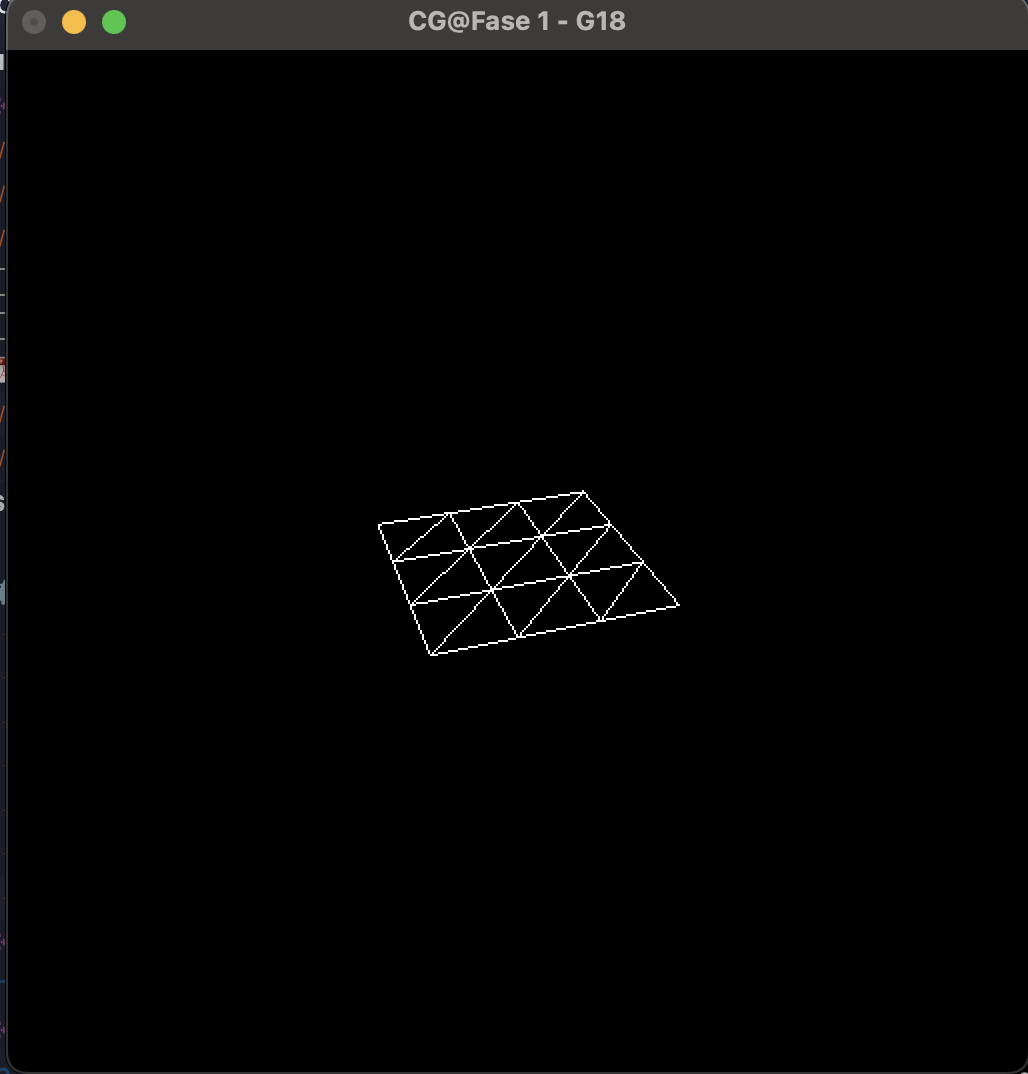
\includegraphics[width=0.5\linewidth]{images/plane_1_3.png}
    \caption{Plano gerado com parâmetros: \textbf{unit} = 1, \textbf{slices} = 3}
    \label{fig:plane-13}
\end{figure}



\textbf{Sphere} \\

A esfera é gerada utilizando coordenadas esféricas. A ideia é dividir a esfera em \textbf{stacks} e \textbf{slices}. 
Cada vértice é calculado com coordenadas esféricas, usando as fórmulas:
\begin{itemize}
    \item \(x = r * sin(\theta) * cos(\theta)\)
    \item \(y = r * cos(\theta)\)
    \item \(z = r * sin(\theta) * sin(\phi)\), onde \(\theta\) é o angulo de latitude (\textbf{stacks} e \(\phi\) é o angulo de longitude (\textbf{slices}). Estas coordenadas geram 2 triângulos para cada quadrado formado pelas linhas de latitude e longitude.
\end{itemize}

\begin{figure} [H]
    \centering
    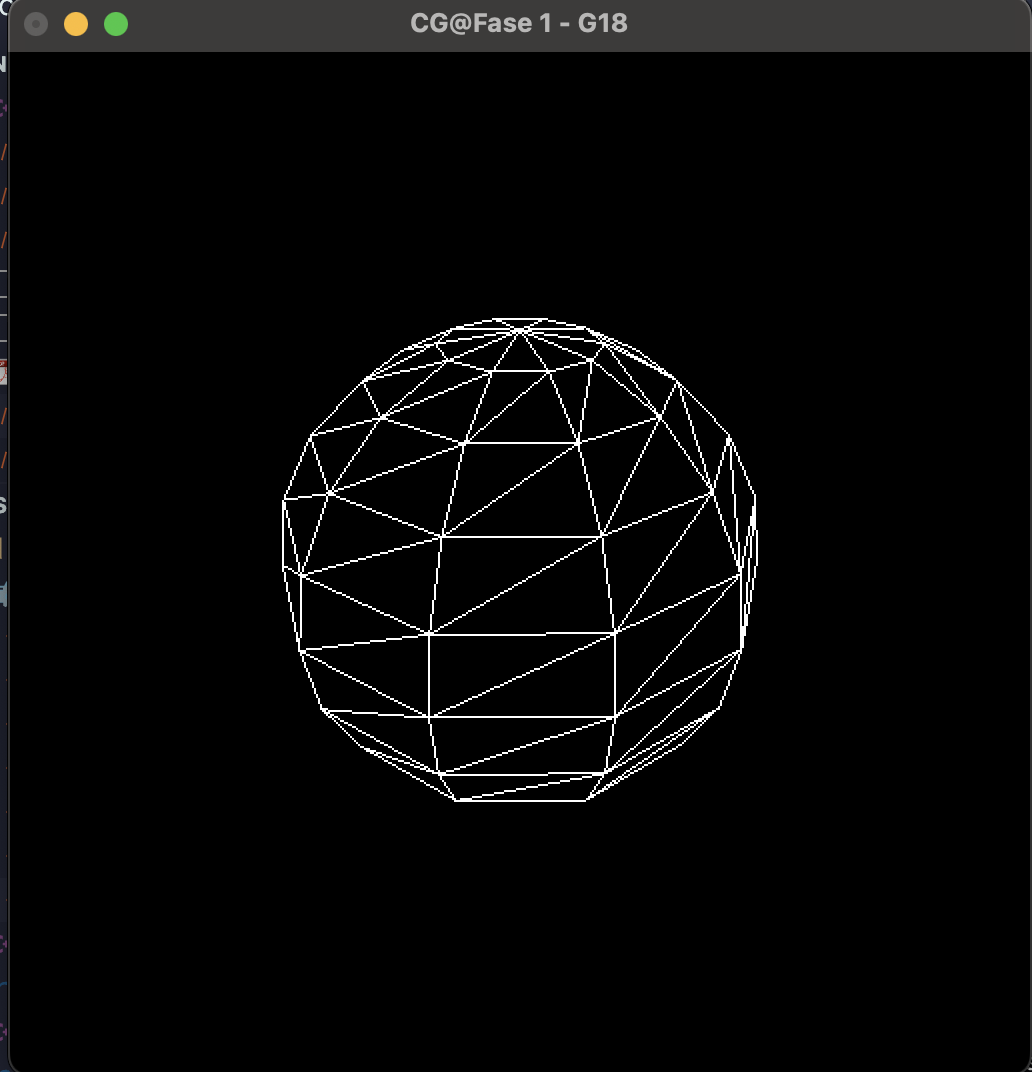
\includegraphics[width=0.5\linewidth]{images/Sphere_1_10_10.png}
    \caption{Esfera gerada com parâmetros: \textbf{radius} = 1, \textbf{slices} = 10, \textbf{stacks} = 10}
    \label{fig:sphere-11010}
\end{figure}

\textbf{Box} \\

A caixa tem 6 faces, e cada face é gerada de forma semelhante ao plano, i.e, é subdividida em triângulos. As faces da caixa são divididas pelas coordenadas dos vértices, e cada face é subdividida em \(i*i\) quadrados, com 2 triângulos cada. 

Para cada face, as coordenadas x, y e z variam de acordo com a face em questão. Utilizamos os valores de comp e \textbf{offset}, apenas ajustando a direção da face (no eixo X, Y ou Z).
\begin{figure} [H]
    \centering
    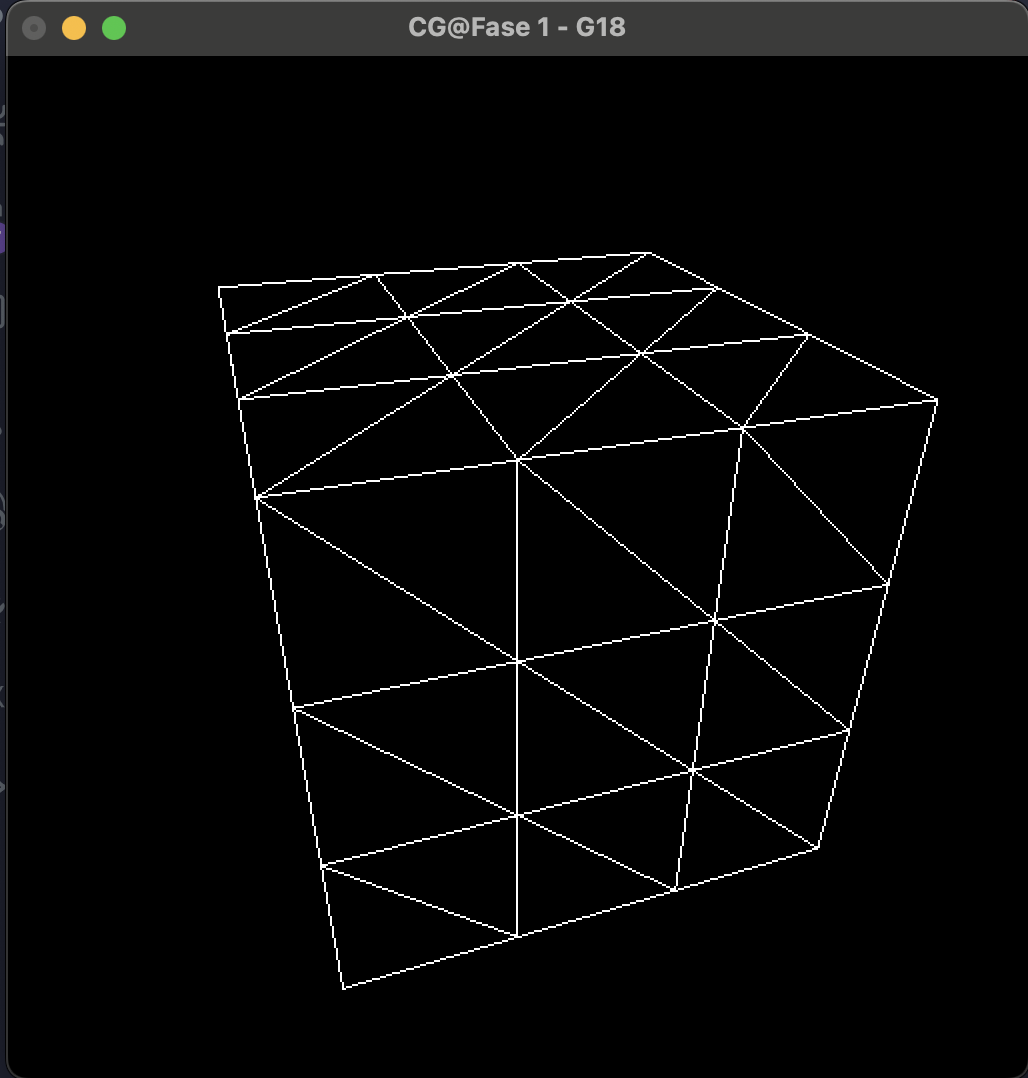
\includegraphics[width=0.5\linewidth]{images/Box_2_3.png}
    \caption{Caixa gerada com parâmetros: \textbf{unit} = 2, \textbf{slices} = 3}
    \label{fig:box-23}
\end{figure}


\textbf{Cone} \\

O cone tem um vértice superior e uma base circular. Para gerar o cone, a base é dividida em \textbf{slices} ao longo da circunferência, e a altura é dividida em camadas (\textbf{stacks}).

Para calcular as coordenadas da base, utilizam-se as coordenadas polares para calcular os pontos na base circular: 
\begin{itemize}
    \item \(x=r*sin(\theta)\)
    \item \(z = r*cos(\theta)\)
\end{itemize}
Cada fatia é representada por 2 triângulos, com o ponto central da base conectado aos pontos da circunferência.

Para as \textbf{stacks} do cone, utilizam-se as coordenadas radiais, mas ajustadas à altura, já que esta diminui à medida em que subimos. 

O cálculo da posição dos vértices nas \textbf{stacks} é dado por \(r=\frac{h}{r_b}\), onde \(r_b\) é o raio da base.
\begin{figure} [H]
    \centering
    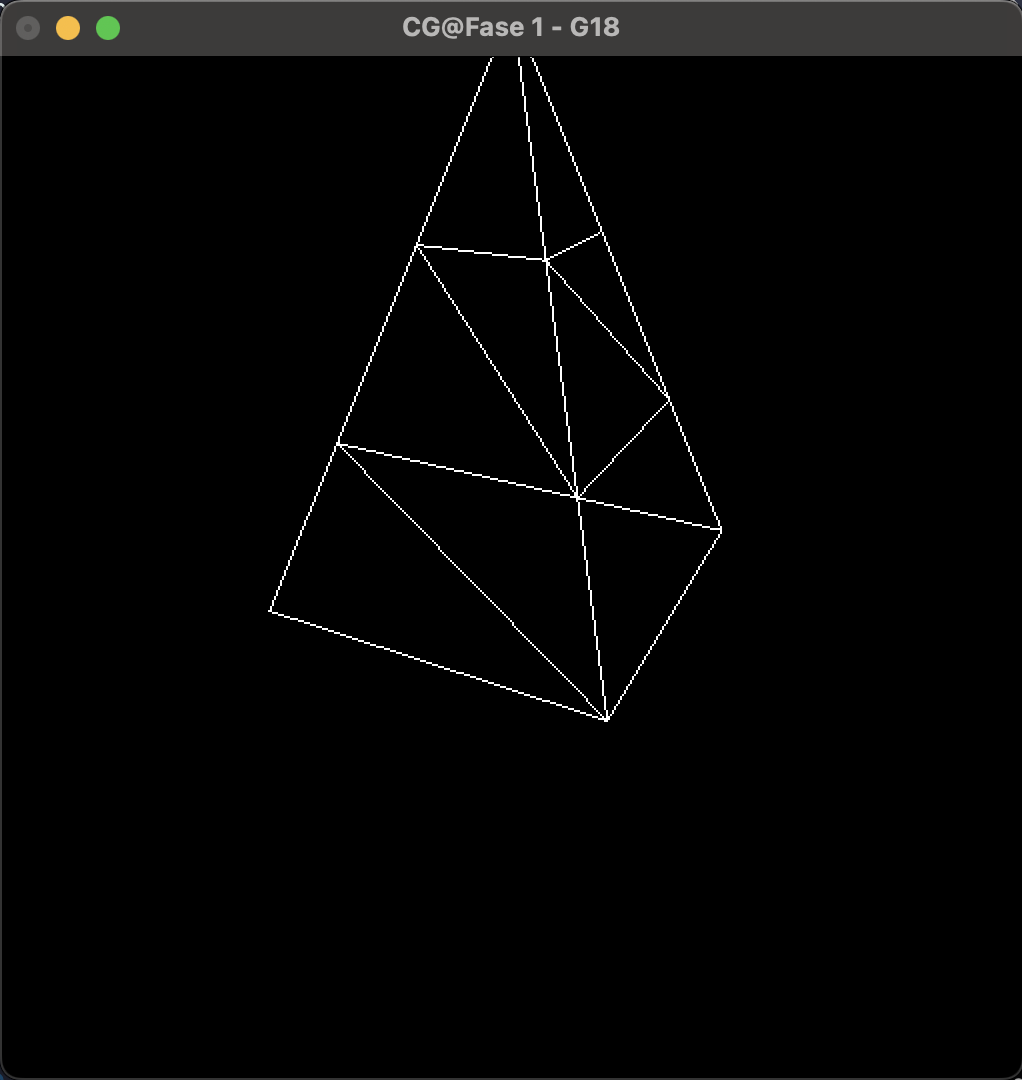
\includegraphics[width=0.5\linewidth]{images/cone_1_2_4_3.png}
    \caption{Cone gerado com parâmetros: \textbf{radius} = 1, \textbf{height} = 2, \textbf{slices} = 4, \textbf{stacks} = 3}
    \label{fig:cone-1243}
\end{figure}


\subsection{Engine}
O \textbf{Engine} é a componente responsável por processar os modelos tridimensionais e exibi-los utilizando o \textbf{OpenGL}. Este programa recebe como parâmetro de entrada um ficheiro \textbf{XML} contendo a configuração da cena, incluindo as definições da câmera, as dimensões da janela e os modelos a serem renderizados. É utilizada a técnica de \textbf{wireframe} para representar as coordenadas dos ficheiros \textbf{.3d}. 

Cada ficheiro começa com um número de triângulos a desenhar e segue com blocos de 4 linhas por triângulo, onde a primeira linha define a cor e as outras 3 as coordenadas dos vértices. Além de ler os modelos, o motor lê um ficheiro \textbf{XML} que configura a cena. O \textbf{XML} é lido utilizando a biblioteca \textbf{TinyXML2}, que extrai as informações necessárias para a renderização. 

A renderização é realizada pela função \textbf{\texttt{renderScene()}}, que limpa o ecrã, configura a câmera, desenha os modelos em \textbf{wireframe} e troca os \textbf{buffers} para exibir uma cena nova. 





\chapter{Instruções de Utilização}\label{chap:instructions}

Para compilar e executar o nosso programa, existem duas formas:

\section{Manualmente}

\begin{enumerate}
    \item Posicionar-se na pasta \texttt{build} com o comando:
    \begin{center}
        \texttt{cd build}
    \end{center}
    \item Executar os seguintes comandos:
    \begin{center}
        \texttt{cmake ..} 
    \end{center}
    seguido de
    \begin{center}
        \texttt{make}
    \end{center}
    \item Posicionar-se na pasta \texttt{generator} e executar o seguinte comando:
    \begin{center}
        \texttt{./generator nome\_figura <parametros> nome\_figura.3d}
    \end{center}
    \item Sair da pasta \texttt{generator} com o comando:
    \begin{center}
        \texttt{cd ..}
    \end{center}
    \item Posicionar-se na pasta \texttt{build} e executar o seguinte comando:
    \begin{center}
        \texttt{./engine ../engine/configs/test\_file\_pretendido.xml}
    \end{center}
\end{enumerate}

\section{Script}

Para simplificar o processo, criámos um \textbf{script} que executa automaticamente todas as instruções mencionadas. Para executar o \textbf{script}, siga os seguintes passos:

\begin{enumerate}
    \item Tornar o \textbf{script} executável com o comando:
    \begin{center}
        \texttt{chmod +x run.sh}
    \end{center}
    \item Executar o \textbf{script} com:
    \begin{center}
        \texttt{./run.sh}
    \end{center}
\end{enumerate}

Após executar o \textbf{script}, será apresentado um menu que permite realizar diversas operações:

\begin{figure} [H]
    \centering
    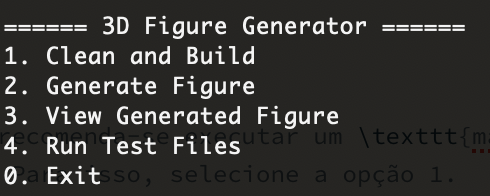
\includegraphics[width=0.5\linewidth]{images/script.png}
    \caption{\textbf{Script} - Menu}
    \label{fig:script-menu}
\end{figure}


\begin{itemize}
    \item Na primeira utilização, recomenda-se executar um \texttt{make clean} e recompilar o projeto. Para isso, seleciona-se a opção \textbf{1}.
    \item Criar objetos 3D utilizando a opção \textbf{2}.
    \item Visualizar os objetos já criados com a opção \textbf{3}.
    \item Executar os ficheiros de teste através da opção \textbf{4}.
\end{itemize}

Dentro da pasta do projeto, incluímos uma pequena demonstração para facilitar a compreensão do processo.

\chapter{Testes} \label{chap:testes}
Nesta secção, serão apresentadas imagens com as figuras renderizadas conforme as configurações dos arquivos de teste no formato \textbf{.XML}.
\begin{enumerate}
    \item \textbf{Teste 1} - Cone gerado com parametros: \textbf{radius} = 1, \textbf{height} = 2, \textbf{slices} = 4, \textbf{stacks} = 3 
    \begin{figure}[H]
    \centering
    \begin{minipage}{0.49\linewidth}
        \centering
        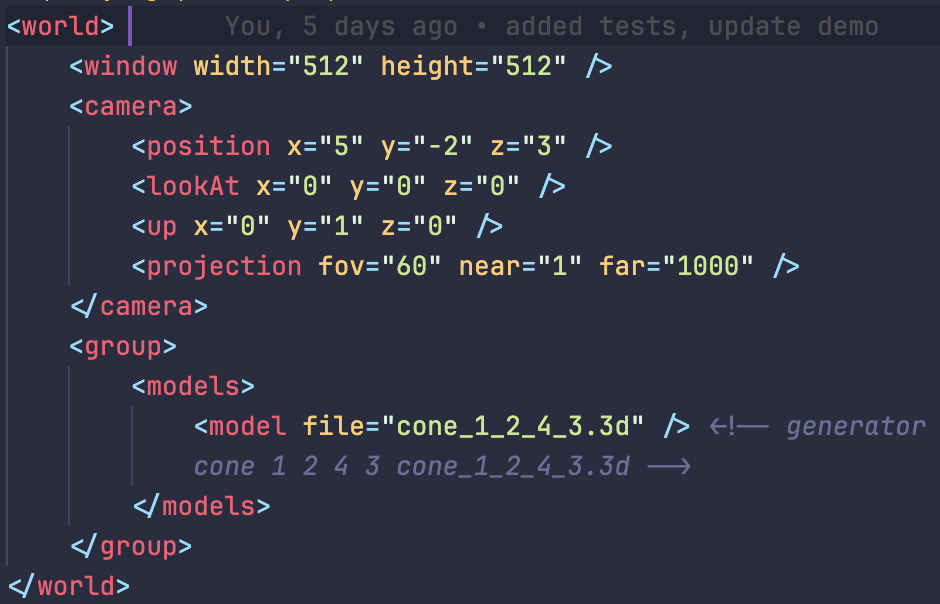
\includegraphics[width=\linewidth]{images/xmlTeste1.png}
        \caption[Teste 1 - XML]{Configuração XML para o Teste 1, onde um cone é gerado com raio 1, altura 2, 4 \textbf{slices} e 3 \textbf{stacks}.}
        \label{fig:xml-teste1}
    \end{minipage}
    \hfill
    \begin{minipage}{0.49\linewidth}
        \centering
        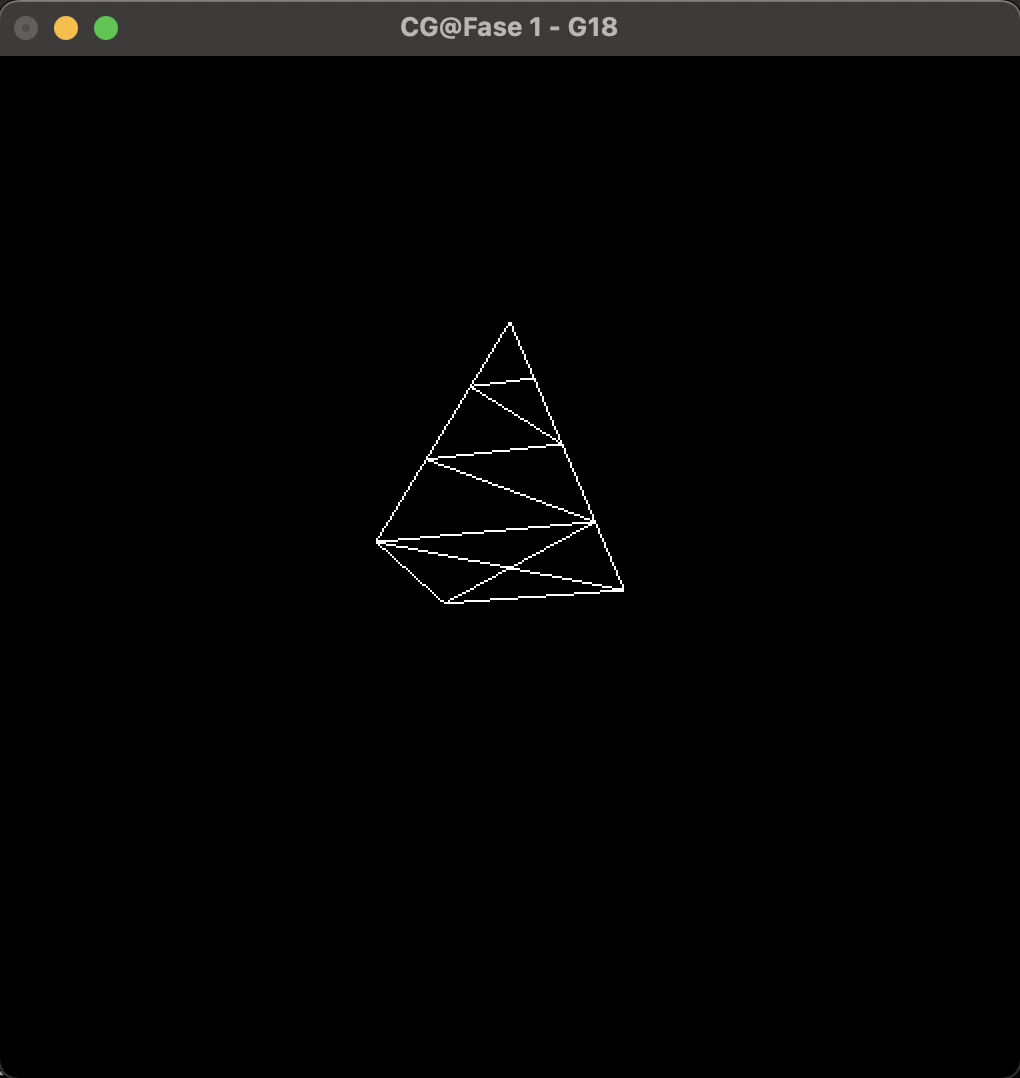
\includegraphics[width=\linewidth]{images/Teste1.png}
        \caption[Teste 1 - Desenho]{Cone renderizado com base na configuração do Teste 1. Observa-se a divisão em 4 \textbf{slices} e 3 \textbf{stacks}.}
        \label{fig:cena-teste1}
    \end{minipage}
\end{figure}
\newpage
    \item \textbf{Teste 2} - Cone gerado com parametros: \textbf{radius} = 1, \textbf{height} = 2, \textbf{slices} = 4, \textbf{stacks} = 3, mas com \textbf{fov} diferente.  
    \begin{figure}[H]
    \centering
    \begin{minipage}{0.49\linewidth}
        \centering
        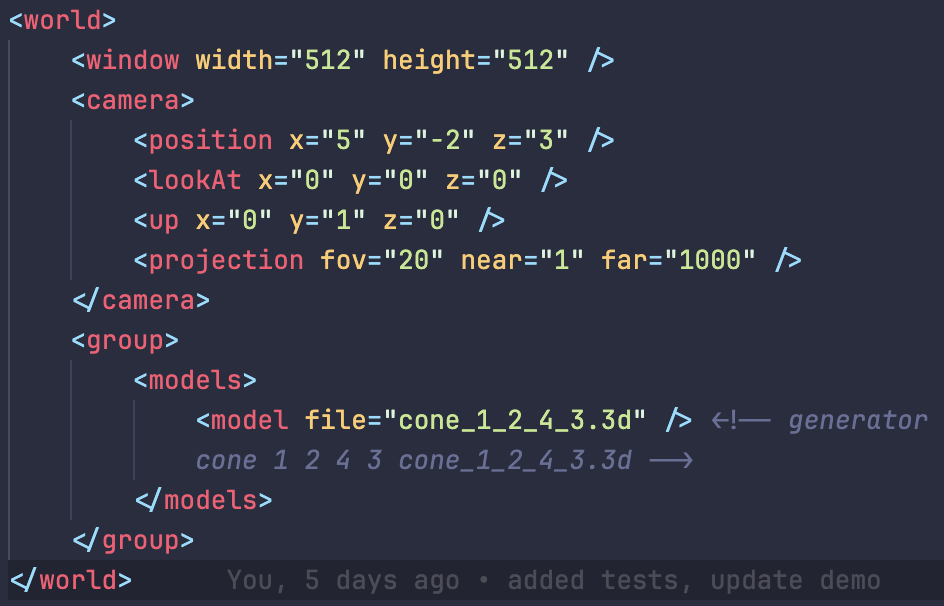
\includegraphics[width=\linewidth]{images/xmlTeste2.png}
        \caption[Teste 2 - XML]{Configuração \textbf{XML} para o Teste 2, onde um cone é gerado com raio 1, altura 2, 4 \textbf{slices} e 3 \textbf{stacks}, mas com um \textbf{fov} diferente}
        \label{fig:xml-teste2}
    \end{minipage}
    \hfill
    \begin{minipage}{0.49\linewidth}
        \centering
        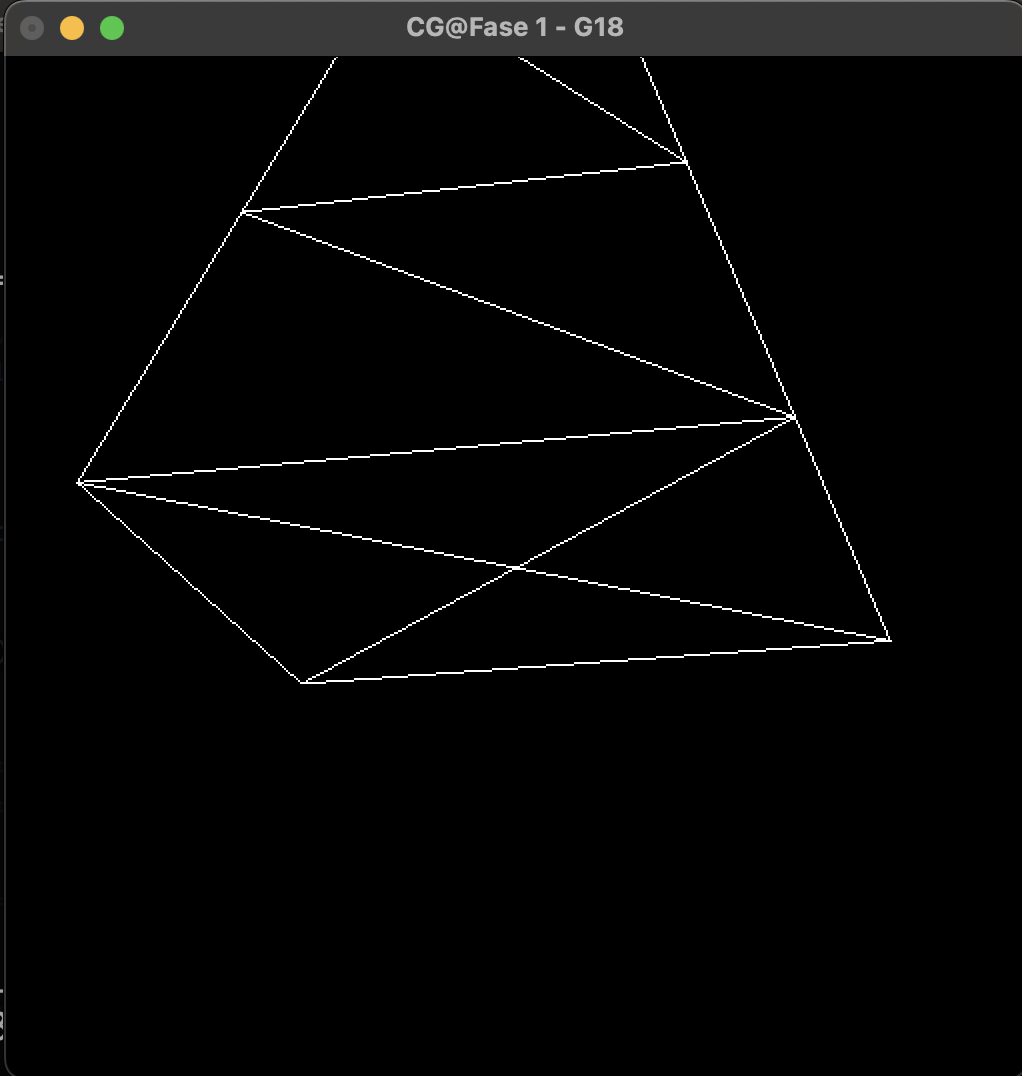
\includegraphics[width=\linewidth]{images/Teste2.png}
        \caption[Teste 2 - Desenho]{Cone renderizado com base na configuração do Teste 2. Observa-se a divisão em 4 \textbf{slices} e 3 \textbf{stacks}.}
        \label{fig:cena-teste2}
    \end{minipage}
\end{figure}

\newpage

\item \textbf{Teste 3} - Esfera gerada com parametros: \textbf{radius} = 1, \textbf{slices} = 10, \textbf{stacks} = 10.  
    \begin{figure}[H]
    \centering
    \begin{minipage}{0.49\linewidth}
        \centering
        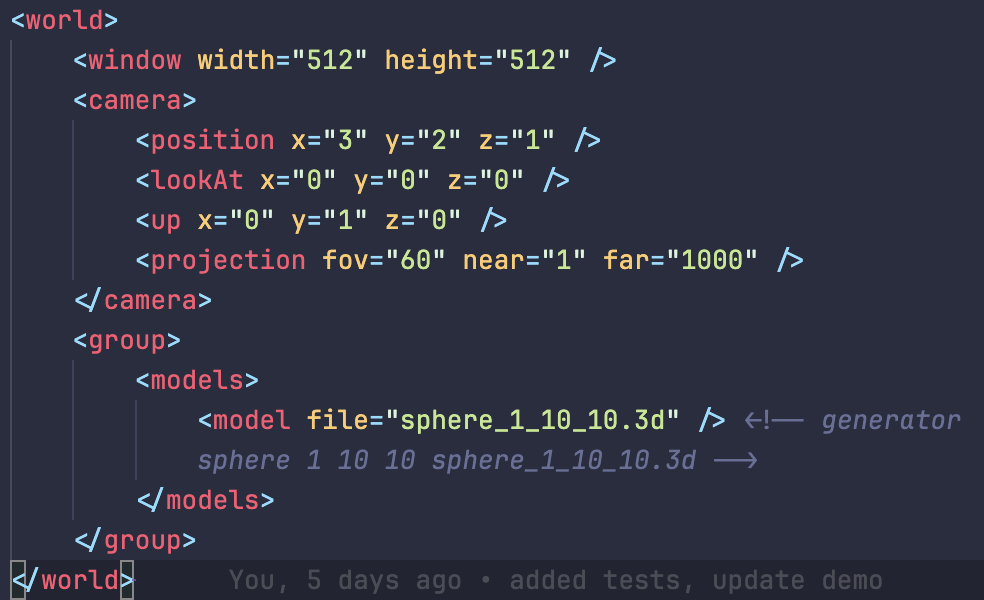
\includegraphics[width=\linewidth]{images/xmlTeste3.png}
        \caption[Teste 3 - XML]{Configuração \textbf{XML} para o Teste 3, onde uma esfera é gerada com raio 1, 10 \textbf{slices} e 10 \textbf{stacks}.}
        \label{fig:xml-teste3}
    \end{minipage}
    \hfill
    \begin{minipage}{0.49\linewidth}
        \centering
        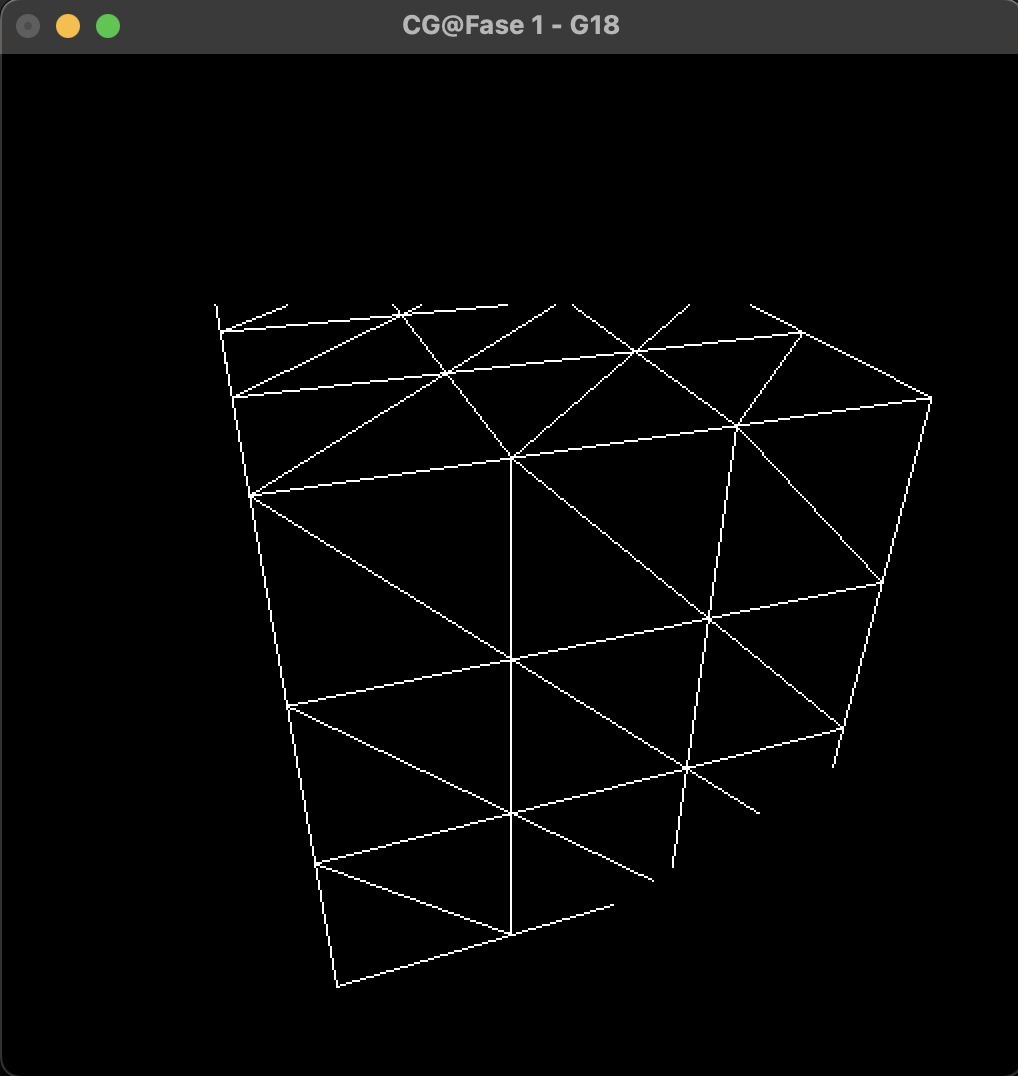
\includegraphics[width=\linewidth]{images/Teste3.png}
        \caption[Teste 3 - Desenho]{Esfera renderizada com base na configuração do Teste 3. Observa-se a divisão em 10 \textbf{slices} e 10 \textbf{stacks}.}
        \label{fig:cena-teste3}
    \end{minipage}
\end{figure}

\newpage

\item \textbf{Teste 4} - Caixa gerada com parametros: \textbf{unit} = 2, \textbf{slices} = 3.
    \begin{figure}[H]
    \centering
    \begin{minipage}{0.49\linewidth}
        \centering
        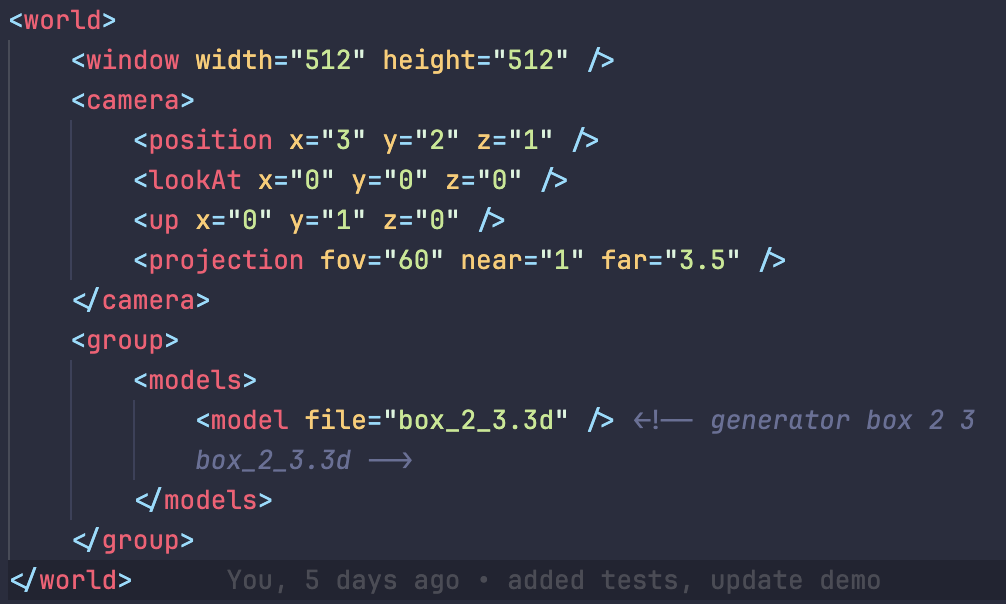
\includegraphics[width=\linewidth]{images/xmlTeste4.png}
        \caption[Teste 4 - XML]{Configuração \textbf{XML} para o Teste 4, onde uma caixa é gerada com arestas de comprimento 2 e 3 \textbf{slices} por face.}
        \label{fig:xml-teste4}
    \end{minipage}
    \hfill
    \begin{minipage}{0.49\linewidth}
        \centering
        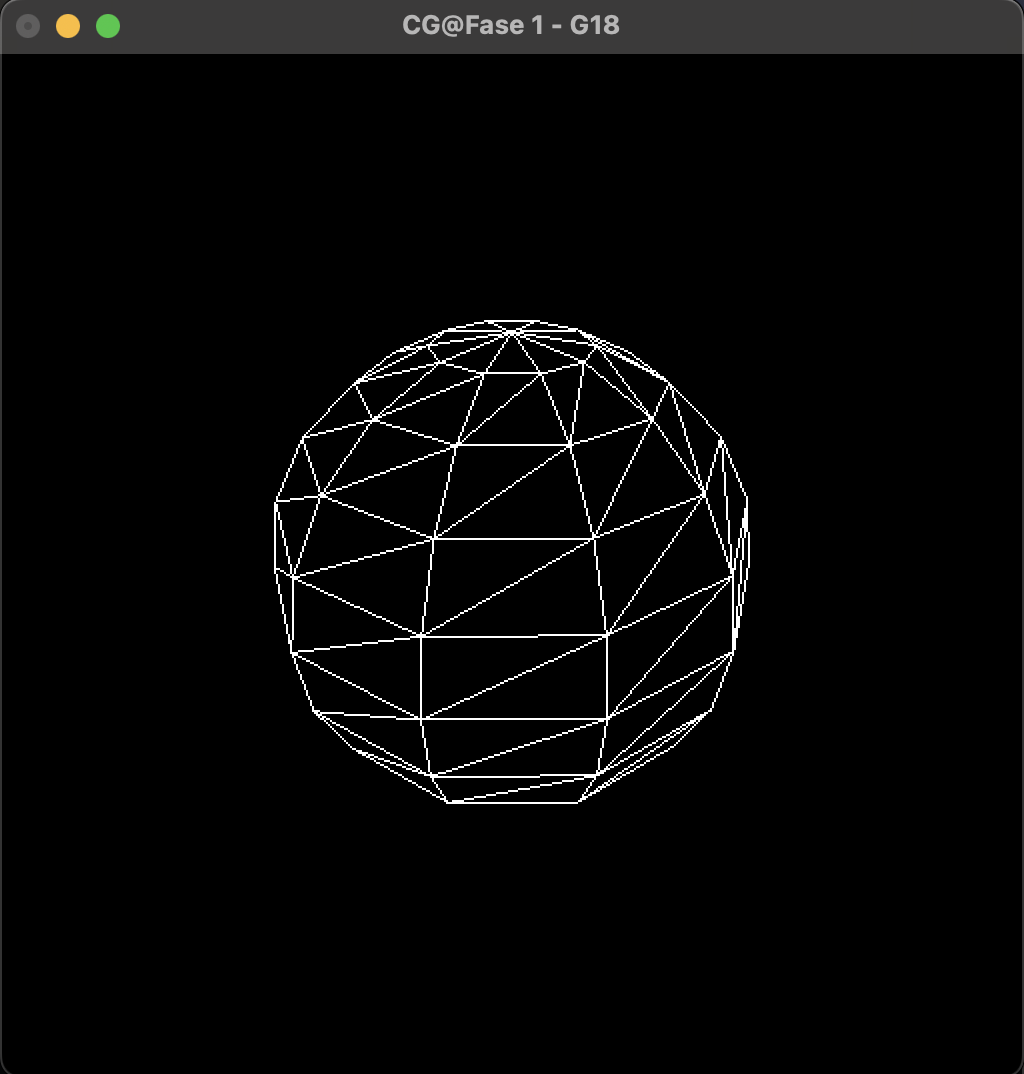
\includegraphics[width=\linewidth]{images/Teste4.png}
        \caption[Teste 4 - Desenho]{Caixa renderizada com base na configuração do Teste 4. Observa-se a divisão em 3 \textbf{slices} por face.}
        \label{fig:cena-teste4}
    \end{minipage}
\end{figure}

\newpage

\item \textbf{Teste 5} - Composição de figuras com um plano e uma esfera.
    \begin{figure}[H]
    \centering
    \begin{minipage}{0.49\linewidth}
        \centering
        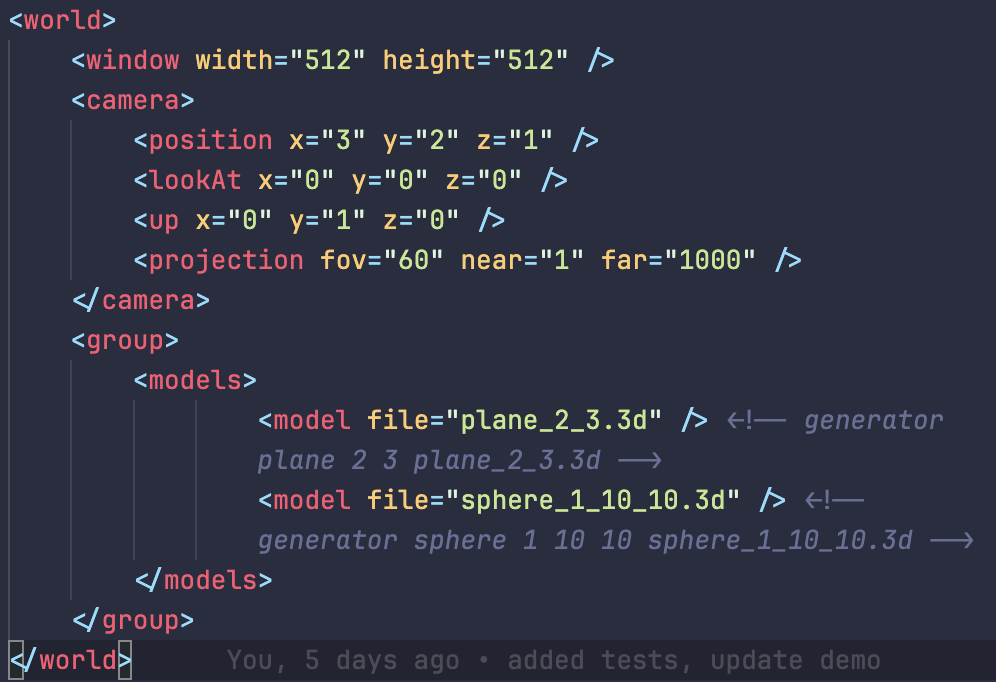
\includegraphics[width=\linewidth]{images/xmlTeste5.png}
        \caption[Teste 5 - XML]{Configuração \textbf{XML} para o Teste 5, onde um plano e uma esfera são renderizados na mesma cena.}
        \label{fig:xml-teste5}
    \end{minipage}
    \hfill
    \begin{minipage}{0.49\linewidth}
        \centering
        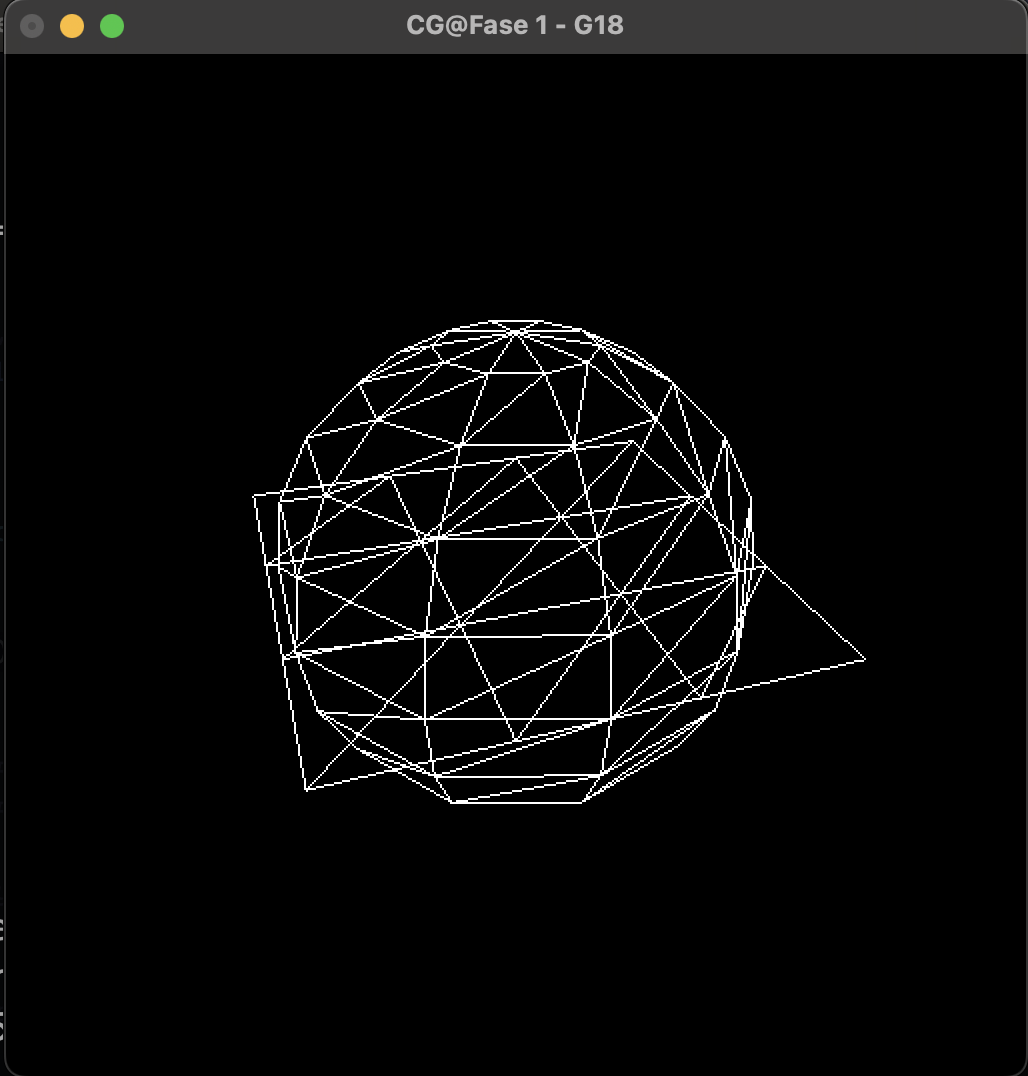
\includegraphics[width=\linewidth]{images/Teste5.png}
        \caption[Teste 5 - Desenho] {Cena renderizada com base na configuração do Teste 5. Observa-se o plano no eixo XZ e a esfera acima dele.}
        \label{fig:cena-teste5}
    \end{minipage}
\end{figure}




\end{enumerate}

\chapter{Conclusão} \label{chap:conclusao}

Nesta primeira fase deste projeto, tivemos oportunidade de aplicar os conceitos descritos ao longo das aulas. 
Observamos a importância da correção das expressões utilizadas para calcular os vértices corretamente antes do desenho das nossas formas geométricas. Chegamos à conclusão que qualquer erro nestes valores, assim como na ordem de geração dos pontos, podiam levar a grandes erros quando se chegava à fase de desenho dos modelos.

Este projeto tem sido uma experiência nova para nós, dado que até este ponto, ainda não tínhamos tido oportunidade de explorar esta área da computação.

Consideramos que o nosso projeto tem os pontos pedidos no enunciado do mesmo, no entanto, nas fases seguintes, esperamos conseguir implementar novas funções, por exemplo, mudar o ângulo de visão dos objetos através de input do teclado ou rato.





\end{document}

\documentclass{article}
\usepackage[utf8]{inputenc}
\usepackage{glossaries}

\makeglossaries

\newglossaryentry{latex}
{
    name=latex,
    description={Is a mark up language specially suited
    for scientific documents}
}

\newglossaryentry{maths}
{
    name=mathematics,
    description={Mathematics is what mathematicians do}
}

\title{How to create a glossary}
\author{ }
\date{ }

\begin{document}
\maketitle

The \Gls{latex} typesetting markup language is specially suitable
for documents that include \gls{maths}.

\clearpage

\printglossaries

\end{document}
